\input{configuration}

\title{Lecture 3 --- Relational Query Languages and SQL}

\author{Jeff Zarnett \\ \small \texttt{jzarnett@uwaterloo.ca}}
\institute{Department of Electrical and Computer Engineering \\
  University of Waterloo}
\date{\today}


\begin{document}

\begin{frame}
  \titlepage

 \end{frame}



\begin{frame}
\frametitle{Relational Query Languages}

A \alert{query language} is a language to get information from the database. 

\begin{center}
	
\includegraphics[width=0.4\textwidth]{images/askaquestion.jpg}
\end{center}
\hfill \textit{``Excuse me, I'd just like to ask a question...''}

 \end{frame}



\begin{frame}
\frametitle{Relational Query Languages}

Procedural: you tell the database exactly how to get the data you want.

Non-procedural: tell the database what you want; it figures out how to deliver.

\end{frame}



\begin{frame}
\frametitle{Relational Query Languages}

Operations can be applied to a single relation, or a pair of relations.

The result of this is always a single relation. 

This means that the output of one operation can be used as the input to another operation, allowing us to chain operations as needed. 

\end{frame}



\begin{frame}
\frametitle{Functions Everywhere!}

If it helps you to imagine this, every operation is a function with return type \texttt{Relation} and they take either one or two \texttt{Relation}s as parameters.

You will also need to keep in mind that because they all have input and output of relation(s), the operations operate on a set of data, not just a single element.


\end{frame}



\begin{frame}
\frametitle{\texttt{if (sql != C)} }

In a C-like language, you write a \texttt{for} loop to sets all elements in an array to \texttt{-1}. 

In SQL, you write a query that sets the value to \texttt{-1} for all entries in the relation. 

\end{frame}



\begin{frame}
\frametitle{\texttt{if (sql != C)} }

This means that if your normal mode of thinking is C-like (procedural) then there is a mental transition that needs to be made. 

\begin{center}
	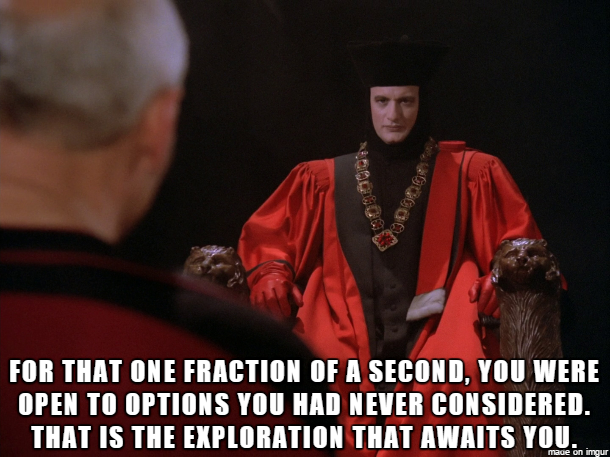
\includegraphics[width=0.7\textwidth]{images/q-agt.png}
\end{center}

\end{frame}



\begin{frame}
\frametitle{Relational Algebra}


The fundamental operations in relational algebra are:
\begin{itemize}
	\item Select
	\item Project
	\item Union
	\item Set Difference
	\item Cartesian Product
	\item Rename
\end{itemize}

\end{frame}



\begin{frame}
\frametitle{Relational Algebra}


And there are three shortcuts we will use that can be created using the fundamental operations: 

\begin{itemize}
	\item Set Intersection
	\item Assignment
	\item Join
\end{itemize}


\end{frame}



\begin{frame}
\frametitle{Ess Cue Ell or Sequel?}

SQL -- ``Structured Query Language'' -- is not only for querying but also for defining and changing the database schema. 

It is a nonprocedural language: you ask for what you want and the database server returns a result that matches that format.

Other query languages do exist.

\end{frame}



\begin{frame}
\frametitle{This is UNIX! I know UNIX!}

Reality check: the majority of students taking this course already have exposure to some form of database system. 

Most likely a SQL relational database of some sort. 

\end{frame}



\begin{frame}
\frametitle{This is UNIX! I know UNIX!}

That means that a course where we spend a lot of time on SQL is redundant.\\
\quad But we can't skip it either... It can still have value.

Still, the mathematical notation may be new.

\end{frame}



\begin{frame}
\frametitle{Making the Sequel}


\begin{itemize}
	\item Data Definition Language (DDL) 
	\item Data Manipulation Language (DML)
	\item Data Control Language (DCL)
	\item Transaction Control Language (TCL)
\end{itemize}


\end{frame}


\begin{frame}
\frametitle{Our Sample Data}

{\small
\begin{center}
\begin{tabular}{|l|l|l|l|l|} \hline
	\textbf{VIN} & \textbf{year} & \textbf{make} & \textbf{model} & \textbf{license\_plate\_number} \\ \hline
	2B4FH25K1RR646348 & 2005 & Honda & Civic & ZZZZ 249 \\ \hline
	4UZACLBW87CZ42980 & 2011 & Ford & Focus & YYYY 995 \\ \hline
	WVWDM7AJ4BW227648 & 2015 & Volkswagen & Golf & ZRHC 112 \\ \hline
	1J4FT38L7KL506678 & 2017 & Audi & A4 & VNTY PLT \\ \hline
	2C8GF48415R447850 & 2016 & Volkswagen & Jetta & VWJG 071 \\ \hline
	2T3RK4DV1AW089914 & 2014 & Toyota & Camry & ZZZZ 385 \\ \hline
	1XPCDR9X2YN436206 & 2012 & Toyota & Camry & ZZYY 251 \\ \hline
	1GYS3BKJ5FR338462 & 2016 & Honda & Civic & YYYY 585 \\ \hline
	1GAGG25R6Y1243081 & 2015 & Chevrolet & Corvette & GORLFAST \\ \hline
	JH2SC59208M054959 & 2018 & Genesis & Genesis & AAAA 123 \\ \hline
\end{tabular}
\end{center}
}


\end{frame}




\begin{frame}
\frametitle{Selection}

The first operation we will discuss is \alert{selection}: find the tuples in the relation.

\begin{center}
	
\includegraphics[width=0.6\textwidth]{images/wantthemalive.jpg}
\end{center}



We need to specify what we want to find, and where we want to look for it. 

We can specify that we want to find only the things that match certain criteria. 


\end{frame}



\begin{frame}
\frametitle{Selection}

In mathematical notation, selection has the symbol $\sigma$ (sigma). 

The predicate is put in a subscript and then the function parameter, the relation to select from, is follows in parenthesis. 

$\sigma_{make = ''Volkswagen''}( vehicle )$:

{\small
\begin{center}
\begin{tabular}{|l|l|l|l|l|} \hline
	\textbf{VIN} & \textbf{year} & \textbf{make} & \textbf{model} & \textbf{license\_plate\_number} \\ \hline
	WVWDM7AJ4BW227648 & 2015 & Volkswagen & Golf & ZRHC 112 \\ \hline
	2C8GF48415R447850 & 2016 & Volkswagen & Jetta & VWJG 071 \\ \hline
\end{tabular}
\end{center}
}

\end{frame}



\begin{frame}
\frametitle{Writing the Predicate}

We specify the predicate $p$ using propositional logic. 

A term is written as an attribute followed by a comparison operator then an attribute or constant. 

The comparison operators are $=, \neq, >, \geq, <, \leq$.

 So the attribute in the example is $make$ and the comparison operator is $=$ (equals) and then the right hand side is the constant ``Volkswagen''. 


\end{frame}



\begin{frame}
\frametitle{Compound Predicate}

Terms are connected by the mathematical AND $\wedge$, mathematical OR $\vee$, and mathematical NOT $\neg$ operators. 

Thus we could specify make = ``Volkswagen'' and year = ``2015'':

($\sigma_{make = ''Volkswagen'' \wedge year = ''2015''}( vehicle )$):

{\small
\begin{center}
\begin{tabular}{|l|l|l|l|l|} \hline
	\textbf{VIN} & \textbf{year} & \textbf{make} & \textbf{model} & \textbf{license\_plate\_number} \\ \hline
	WVWDM7AJ4BW227648 & 2015 & Volkswagen & Golf & ZRHC 112 \\ \hline
\end{tabular}
\end{center}
}


\end{frame}



\begin{frame}
\frametitle{Compound Predicate}

We can chain as many of these qualifiers as desired. 

Use of parenthesis is recommended to make it clear how the boolean logic is to be evaluated. 

If you wish the year to be either 2015 or 2016 and the make to be Volkswagen:

$make = ''Volkswagen'' \wedge ( year = ''2015'' \vee year = ''2016'' )$.

It doesn't cost extra money to write the parenthesis so use them anywhere there is the possibility of error or confusion. 


\end{frame}



\begin{frame}
\frametitle{Empty-Handed}

It is possible that no tuples in the relation match all of the predicates. 

If the predicate is make = ``Chrysler'' then no matches will be found. 

If we specify make = ``Honda'', and model = ``Camry'', we will still find no tuples that match that either. Honda doesn't manufacture any model named ``Camry''.

Either way we get back an empty relation.


\end{frame}




\begin{frame}
\frametitle{Selection in SQL}

In SQL, the \texttt{SELECT} clause is used to, well, select tuples from the database. 

The SQL command corresponding to $\sigma( vehicle )$ is \texttt{SELECT * FROM VEHICLE;} 

\end{frame}




\begin{frame}
\frametitle{Selection in SQL}

It is traditional in SQL that we write keywords in all capitals.

A statement is terminated by a semicolon. 

Note the use of \texttt{FROM} to specify the relation. 

The asterisk (\texttt{*}) is needed to specify what we are going to select.
\end{frame}



\begin{frame}
\frametitle{Selection in SQL}

The select statement contains no predicates so it would return all tuples in the relation. 

\texttt{SELECT * FROM VEHICLE WHERE make = 'Volkswagen';}

The \texttt{WHERE} keyword indicates the start of the predicate. 

The string literal ``Volkswagen'' is enclosed in single quotation marks but it can also be in double quotation marks  

To form a compound predicate: \texttt{SELECT * FROM VEHICLE WHERE make = 'Volkswagen' AND year = '2015';}. 


\end{frame}



\begin{frame}
\frametitle{SQL Predicate Comparison}

The comparison operators \texttt{<, >, >=, <=} all look like C. 

Equals is just a single equals sign (\texttt{=}). 

The not equals operator is written \texttt{<>}. 

These operations can work on strings, mathematical types, dates, et cetera. 

You may get unexpected results if you attempt to compare two types that don't compare well.

\end{frame}



\begin{frame}
\frametitle{Range in a Predicate}

It is possible to chain the where clause to include a range, such as \texttt{WHERE year >= 2010 AND year <= 2015}.

there is a bit of notational convenience in SQL: the \texttt{BETWEEN ... AND} syntax. 

Thus one can write \texttt{WHERE year BETWEEN 2010 AND 2015}. 

This is inclusive on both ends, so be careful about whether this is the desired behaviour. 

\end{frame}



\begin{frame}
\frametitle{Use of Attributes}

The predicate may also contain the name of other attributes in the relation.

\texttt{SELECT * FROM VEHICLE WHERE make = model;}. 

This returns the 1 tuple in the sample data where make and model are the same. 

There are situations in real life where we want to use an attribute rather than a constant, although in this particular example it may look a little strange.

\end{frame}



\begin{frame}
\frametitle{Projection}

The second operation is \alert{projection}. 

\begin{center}
	
\includegraphics[width=0.7\textwidth]{images/projection.jpg}
\end{center}

This takes a subset of a relation: take a relation and extract from it only the things that we asked for. 

\end{frame}



\begin{frame}
\frametitle{Projection}

Projection cuts down the relation to the specific attributes. 

Projection takes a single relation and returns another relation.


\end{frame}



\begin{frame}
\frametitle{Projection}

If we want to know what the VIN is for the car with the license plate ``GORLFAST'' we can ask for just that and need not get back the entire tuple. 

Similarly, if you want to get a list of the makes and models in the database, again, it's nice to be able to get this data without any parts you do not need. 

Projection also makes certain things a lot faster: it makes no sense to load all this extra data to your program just to ignore almost all the columns.

\end{frame}



\begin{frame}
\frametitle{Projection}

In mathematical notation, projection has the symbol $\Pi$ (capital pi). 

Like selection, it takes a subscript and the input relation follows in parenthesis. 

So, $\Pi_{make, model}( vehicle )$ will reduce the relation down to just the attributes make and model, leaving out VIN, year, and license plate number information.

All tuples in the relation will appear in the output of the projection operation, although it is entirely possible that some of them look very much alike. 

\end{frame}



\begin{frame}
\frametitle{Projected Vehicle Table}

\begin{center}
\begin{tabular}{|l|l|} \hline
\textbf{make} & \textbf{model} \\ \hline
	Honda & Civic \\ \hline
	Ford & Focus \\ \hline
	Volkswagen & Golf \\ \hline
	Audi & A4  \\ \hline
	Volkswagen & Jetta  \\ \hline
	Toyota & Camry \\ \hline
	Chevrolet & Corvette \\ \hline
	Genesis & Genesis \\ \hline
\end{tabular}
\end{center}

\end{frame}



\begin{frame}
\frametitle{No Duplicates}

There are fewer tuples in this relation than there were in the original relation. 

Remember: a relation is a set and therefore duplicates are not permitted. 

The order of the tuples is not specified either. 

The attributes will be listed in the order they are provided in the project clause, which we may choose arbitrarily. 

\end{frame}




\begin{frame}
\frametitle{Projection in SQL}
In SQL projection is done through our application of the \texttt{SELECT} clause. 

In the previous examples we used \texttt{*} which specified all attributes. 

In production code, the use of \texttt{SELECT *} is discouraged.

\end{frame}



\begin{frame}
\frametitle{Projection in SQL}

\texttt{SELECT make, model FROM VEHICLE;}  returns:

\begin{center}
\begin{tabular}{|l|l|} \hline
	\textbf{make} & \textbf{model} \\ \hline
	Honda & Civic \\ \hline
	Ford & Focus \\ \hline
	Volkswagen & Golf \\ \hline
	Audi & A4  \\ \hline
	Volkswagen & Jetta \\ \hline
	Toyota & Camry  \\ \hline
	Toyota & Camry  \\ \hline
	Honda & Civic  \\ \hline
	Chevrolet & Corvette  \\ \hline
	 Genesis & Genesis \\ \hline
\end{tabular}
\end{center}


\end{frame}



\begin{frame}
\frametitle{Department of Redundancy Department}

Detection of duplicates is relatively difficult (computationally expensive).

SQL does not remove them unless you ask, so technically what you get back is more akin to a list than to a set. 

If you wish to remove duplicates you may use the keyword \texttt{DISTINCT}:\\\texttt{SELECT DISTINCT make, model FROM VEHICLE;}.

The opposite of \texttt{DISTINCT} is the \texttt{ALL} keyword, but since this is the default behaviour you are unlikely to need to write it.

\end{frame}



\begin{frame}
\frametitle{Select Does Two Things}

The SQL \texttt{SELECT} statement is then both selection and projection. 

In what order do these operations take place? Sometimes it does not matter, e.g., if we asked for \texttt{SELECT *...} then the projection does nothing. 

Here's a hint: this statement is perfectly valid: \texttt{SELECT make, model from VEHICLE WHERE year = '2016';} and returns: 

\begin{center}
\begin{tabular}{|l|l|} \hline
\textbf{make} & \textbf{model} \\ \hline
	Volkswagen & Jetta  \\ \hline
	Honda & Civic \\ \hline
\end{tabular}
\end{center}


\end{frame}



\begin{frame}
\frametitle{Find and Reduce}

Clearly the selection operation must take place first! 

If we cut the attributes down to just make and model, then we lose the information we need to tell whether the year is 2016 or not. 

\end{frame}


 

\begin{frame}
\frametitle{Fun with Selection}

The \texttt{SELECT} statement in SQL lets us do some interesting things other than select attributes alone. 

The select clause may contain arithmetic expressions using the operators $+, -, *, /$ operating on either attributes or tuples. 

Thus, to get a 2 digit date out of a 4 digit date we could do: \texttt{SELECT year - 2000 FROM VEHICLE;}.

\end{frame}



\begin{frame}
\frametitle{Selecting Constants}

We can also select constants: write that constant instead of the name of the attribute. 

\texttt{SELECT 'Car', make, model FROM vehicle WHERE year = '2016';} produces:

\begin{center}
\begin{tabular}{|l|l|l|} \hline
\textbf{Car} & \textbf{make} & \textbf{model} \\ \hline
	Car & Volkswagen & Jetta  \\ \hline
	Car &Honda & Civic \\ \hline
\end{tabular}
\end{center}


\end{frame}



\begin{frame}
\frametitle{Union}

We can combine two relations using the \alert{union} operation. 

It takes two relations and produces a single relation from them. 

The mathematical symbol is $\cup$, the same as the mathematical set union operator.

Typically this is used in conjunction with other operations (selection, projection) to get the data that you want.

\end{frame}



\begin{frame}
\frametitle{Union in Relational Algebra}

The query $\sigma_{make = ''Ford''}( vehicle ) \cup  \sigma_{make = ''Audi''}( vehicle )$ produces the results: 

{\small
\begin{center}
\begin{tabular}{|l|l|l|l|l|} \hline
	\textbf{VIN} & \textbf{year} & \textbf{make} & \textbf{model} & \textbf{license\_plate\_number} \\ \hline
	4UZACLBW87CZ42980 & 2011 & Ford & Focus & YYYY 995 \\ \hline
	1J4FT38L7KL506678 & 2017 & Audi & A4 & VNTY PLT \\ \hline
\end{tabular}
\end{center}
}


\end{frame}



\begin{frame}
\frametitle{Union in SQL}

In SQL the keyword is \texttt{UNION}. 

Use of parenthesis is recommended (if not mandatory) to help the SQL query parser figure out what it is you are asking for.


\texttt{(SELECT license\_plate\_number FROM vehicle WHERE make = 'Ford') UNION (SELECT license\_plate\_number FROM vehicle WHERE make = 'Audi');}

By why not write this as a compound predicate?

\end{frame}



\begin{frame}
\frametitle{Why Union?}

Union is for when we want to combine data from two different relations.


$(\Pi_{name, street, city, province, postal\_code}(\sigma( owner\_address) )) \cup  (\Pi_{name, street, city, province, postal\_code}(\sigma( employee ) ))$

In SQL:

\texttt{(SELECT name, street, city, province, postal\_code FROM owner\_address)\\ 
UNION\\ 
(SELECT name, street, city, province, postal\_code FROM employee);}


\end{frame}



\begin{frame}
\frametitle{Unite!}

The union operation can only succeed if the types are compatible. 

For the union operation to make sense, two conditions must hold:

\begin{enumerate}
	\item The relations must have the same number of attributes.
	\item The domain of attribute $i$ in the first relation must be the same as the domain of attribute $i$ in the second relation, for all $i$. 
\end{enumerate}

\end{frame}



\begin{frame}
\frametitle{Select with a Constant}

This example also is a situation where we might make use of a selection with a constant. 

If we wanted to produce a relation with all addresses, and wish to include some type information, we could do this:

\texttt{(SELECT 'Vehicle Owner', name, street, city, province, postal\_code FROM owner\_address)\\
UNION\\
(SELECT 'MTO Employee', name, street, city, province, postal\_code FROM employee);}

{\scriptsize
\begin{center}
	\begin{tabular}{|l|l|l|l|l|l|}\hline
		\textbf{} & \textbf{name} &\textbf{street} & \textbf{city} & \textbf{province} & \textbf{postal\_code} \\ \hline
		Vehicle Owner & Jean Valjean & 19 Rue des Prisonniers & Ottawa & ON & B1B 1B1\\ \hline
		Vehicle Owner & Thomas Anderson & 1234 Main St & Waterloo & ON & A0A 0A0\\ \hline
		Vehicle Owner & Alice Jones & 4 Generic Place & Kenora & ON & C2C 2C2\\ \hline
		MTO Employee & Kim Morgan & 491 Example Road & Waterloo & ON & N2N 2N2\\ \hline
		MTO Employee & Jordan Singh & 24 Eastern Avenue & London & ON & N6A 0B0\\ \hline
	\end{tabular}
\end{center}
}


\end{frame}






\end{document}

